\documentclass[10pt, a5paper]{article}
\usepackage{pdfpages}
\usepackage{parallel}
\usepackage[T2A]{fontenc}
\usepackage{ucs}
\usepackage[utf8x]{inputenc}
\usepackage[polish,english,russian]{babel}
\usepackage{hyperref}
\usepackage{rotating}
\usepackage[inner=2cm,top=1.8cm,outer=2cm,bottom=2.3cm,nohead]{geometry}
\usepackage{listings}
\usepackage{graphicx}
\usepackage{wrapfig}
\usepackage{longtable}
\usepackage{indentfirst}
\usepackage{array}
\newcolumntype{P}[1]{>{\raggedright\arraybackslash}p{#1}}
\frenchspacing
\usepackage{fixltx2e} %text sub- and superscripts
\usepackage{icomma} % коскі ў матэматычным рэжыме
\PreloadUnicodePage{4}

\newcommand{\longpage}{\enlargethispage{\baselineskip}}
\newcommand{\shortpage}{\enlargethispage{-\baselineskip}}

\def\switchlang#1{\expandafter\csname switchlang#1\endcsname}
\def\switchlangbe{
\let\saverefname=\refname%
\def\refname{Літаратура}%
\def\figurename{Іл.}%
}
\def\switchlangen{
\let\saverefname=\refname%
\def\refname{References}%
\def\figurename{Fig.}%
}
\def\switchlangru{
\let\saverefname=\refname%
\let\savefigurename=\figurename%
\def\refname{Литература}%
\def\figurename{Рис.}%
}

\hyphenation{admi-ni-stra-tive}
\hyphenation{ex-pe-ri-ence}
\hyphenation{fle-xi-bi-li-ty}
\hyphenation{Py-thon}
\hyphenation{ma-the-ma-ti-cal}
\hyphenation{re-ported}
\hyphenation{imp-le-menta-tions}
\hyphenation{pro-vides}
\hyphenation{en-gi-neering}
\hyphenation{com-pa-ti-bi-li-ty}
\hyphenation{im-pos-sible}
\hyphenation{desk-top}
\hyphenation{elec-tro-nic}
\hyphenation{com-pa-ny}
\hyphenation{de-ve-lop-ment}
\hyphenation{de-ve-loping}
\hyphenation{de-ve-lop}
\hyphenation{da-ta-ba-se}
\hyphenation{plat-forms}
\hyphenation{or-ga-ni-za-tion}
\hyphenation{pro-gramming}
\hyphenation{in-stru-ments}
\hyphenation{Li-nux}
\hyphenation{sour-ce}
\hyphenation{en-vi-ron-ment}
\hyphenation{Te-le-pathy}
\hyphenation{Li-nux-ov-ka}
\hyphenation{Open-BSD}
\hyphenation{Free-BSD}
\hyphenation{men-ti-on-ed}
\hyphenation{app-li-ca-tion}

\def\progref!#1!{\texttt{#1}}
\renewcommand{\arraystretch}{2} %Іначай формулы ў матрыцы зліпаюцца з лініямі
\usepackage{array}

\def\interview #1 (#2), #3, #4, #5\par{

\section[#1, #3, #4]{#1 -- #3, #4}
\def\qname{LVEE}
\def\aname{#1}
\def\q ##1\par{{\noindent \bf \qname: ##1 }\par}
\def\a{{\noindent \bf \aname: } \def\qname{L}\def\aname{#2}}
}

\def\interview* #1 (#2), #3, #4, #5\par{

\section*{#1\\{\small\rm #3, #4. #5}}

\def\qname{LVEE}
\def\aname{#1}
\def\q ##1\par{{\noindent \bf \qname: ##1 }\par}
\def\a{{\noindent \bf \aname: } \def\qname{L}\def\aname{#2}}
}

\begin{document}
\title{Уменьшение простоя (downtime) при обновлении сетевого приложения}
\author{Aliaksandr Kharkevich, Gomel, Belarus\footnote{\url{other.bigmouse@gmail.com}, \url{http://lvee.org/ru/abstracts/147}}}
\maketitle
\begin{abstract}
Continuous availability is an absolute priority for the network applications. However, there are cases when the application is unavailable to users (eg. software update). 
This publication offers one of possible solutions.
\end{abstract}
\begin{quotation}
В связи с релизом nginx 1.9.0, в котором была добавлена возможность балансировки любых приложений работающих через TCP, дальнейший материал справедлив не только к веб"=ресурсам, но и к любым другим, работающим поверх TCP (СУБД, системам аутентификации, каталогам LDAP, VoIP"=системам и т.~п.).
\end{quotation}

При обновлениях, да и при некоторых других работах, простой (downtime) для сетевого приложения является неизбежным злом. Но с ним нужно и можно бороться.

Для примера рассмотрим простейший случай, как на рисунке ниже:

\begin{figure}[h!]
  \centering
  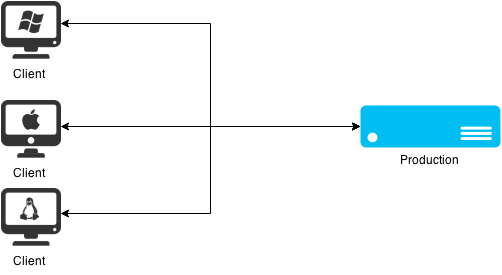
\includegraphics[scale=0.36]{02_2015_01_example}
\end{figure}


Имеется некое клиент"=серверное приложение, и периодически возникает задача его обновлять. При обновлениях возникает время простоя, пользователи выражают недовольство и перестают пользоваться данным приложением (заходить на сайт, оставлять заявки с службу технической поддержки и т.~п.).

Первым этапом в улучшении приложения стала модификация сетевой инфраструктуры "--- добавился сервер для тестирования обновлений, так называемый \emph{staging"=сервер}:

~

\begin{figure}[h!]
  \centering
  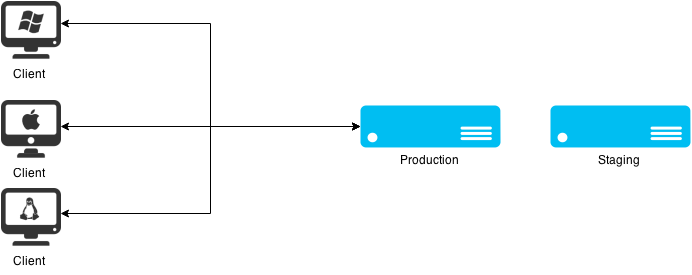
\includegraphics[scale=0.36]{02_2015_02_staging}
\end{figure}

Стало лучше, возможность успешной установки обновлений предварительно проверялась, проверялась и работоспособность основных функций приложения после обновления. Время простоя уменьшилось (как и недовольство пользователей), но не исчезло.

Следующим этапом в улучшении стало добавление обратного прокси в структуру приложения:

~

\begin{figure}[h!]
  \centering
  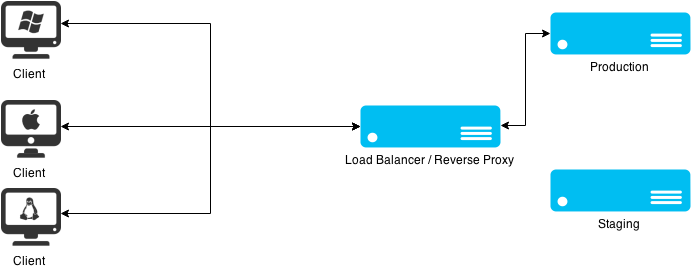
\includegraphics[scale=0.36]{02_2015_03_working}
\end{figure}

Данная структура обеспечила возможность горизонтального масштабирования системы и позволила гибко переключаться между серверами при необходимости (ликвидировать простои на время обслуживания).


Изначально было решено поступить следующим образом: при подготовке сервера к обновлению происходит синхронизация данных на staging"=сервер, затем на нем происходит обновление приложения и основная проверка работоспособности:


\begin{figure}[h!]
  \centering
  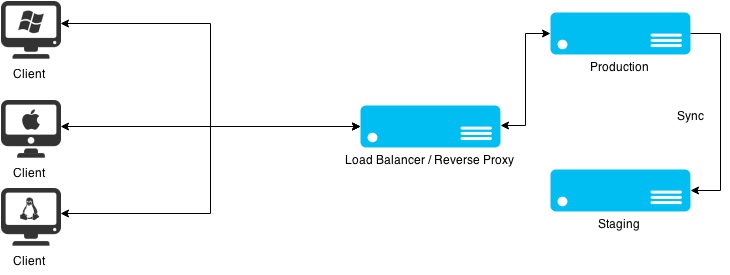
\includegraphics[scale=0.35]{02_2015_04_sync_to_stage}
\end{figure}

Затем происходит переключение обратного прокси на staging"=сервер, переключение длится несколько секунд (из серьезных недостатков "--- мы теряем все активные сессии пользователей). В остальном "--- для конечного пользователя вообще ничего не меняется.

\begin{figure}[h!]
  \centering
  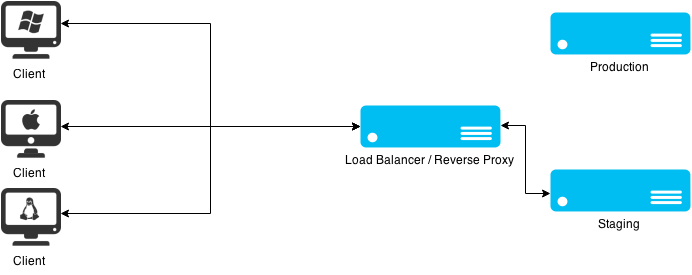
\includegraphics[scale=0.35]{02_2015_05_work_on_stage}
\end{figure}

После переключения нагрузки на staging"=сервер, на \emph{production"=сервере} обновляется приложение. После успешного обновления и проверки его жизнеспособности начинается синхронизация данных со staging (теоретически конечные пользователи уже внесли изменения в данных приложения).

\begin{figure}[h!]
  \centering
  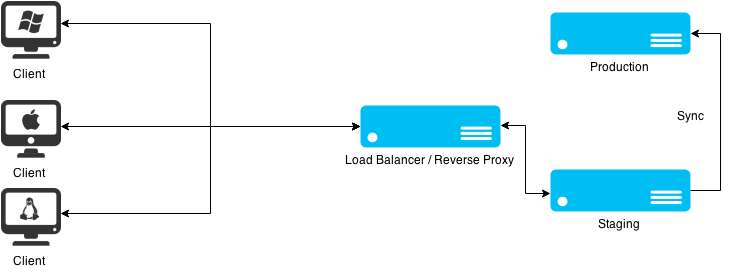
\includegraphics[scale=0.35]{02_2015_06_sync_to_prod}
\end{figure}

После окончания синхронизации происходит переключение обратного прокси"=сервера обратно на production"=сервер.

\begin{figure}[h!]
  \centering
  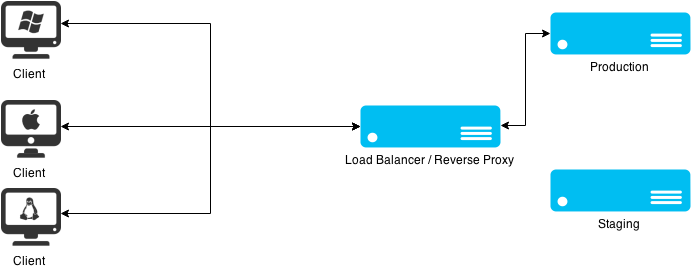
\includegraphics[scale=0.36]{02_2015_07_working_on_prod}
\end{figure}

Но при тестировании на реальных данных нашелся небольшой процент пользователей который изменял данные в момент после синхронизации данных и до переключения между серверами.
В связи с этим, было решено изменить механизм работы приложения.

Был разработан механизм, переводивший приложение в режим <<только чтение>> и уведомлявший пользователей. Перед обновлением production"=сервер переводился в режим <<только чтение>>.

\begin{figure}[h!]
  \centering
  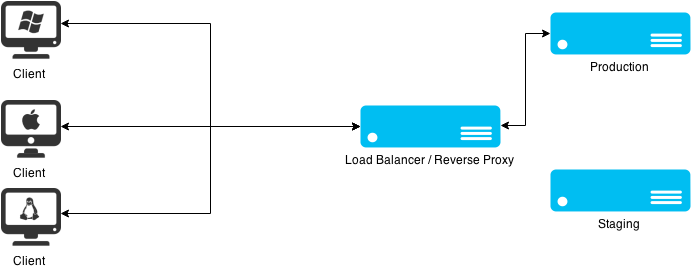
\includegraphics[scale=0.36]{02_2015_08_working}
\end{figure}

После этого происходила синхронизация на staging"=сервер. Приложение на staging"=сервере также в режиме <<только чтение>>.

\begin{figure}[h!]
  \centering
  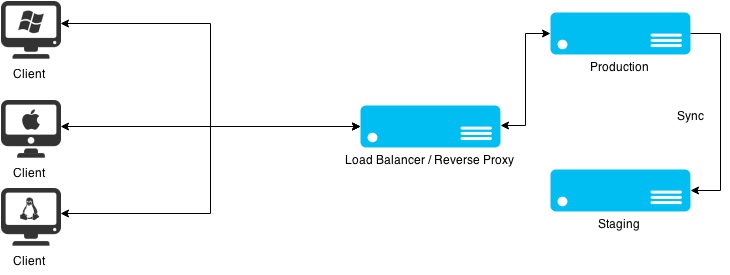
\includegraphics[scale=0.36]{02_2015_09_sync_to_stage}
\end{figure}

После этих манипуляций происходит переключение production"=прокси на staging, и при этом мы убрали вероятность потери данных в момент синхронизации"=переключения. Пользователи получили доступ к приложению и его данным только на чтение на момент обновления, количество негативных отзывов стало минимальным за все время (все отнеслись с пониманием к надписи, предупреждающей о технических работах). Далее "--- переключение приложения на staging, обновление production"=сервера, переключение обратно, и лишь затем "--- отключение режима <<только чтение>>.

\begin{figure}[h!]
  \centering
  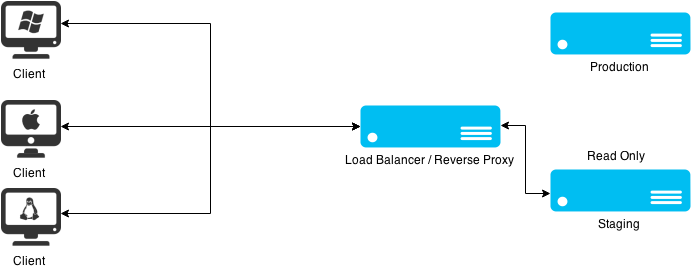
\includegraphics[scale=0.36]{02_2015_10_readonly_work_on_stage}
\end{figure}

\subsection*{Вместо заключения}

Мы добились высокой доступности приложения. При этом, синхронизация данных максимально упрощена, необходимости в изменении работы логики приложения нет (что в свою очередь позволяет ее применять к уже существующим решениям без добавления / изменения логики работы).

\end{document}
